\chapter{Opis projektnog zadatka}
	
	

\begin{comment}

		\textbf{\textit{dio 1. revizije}}\\
        		
		\textit{Na osnovi projektnog zadatka detaljno opisati korisničke zahtjeve. Što jasnije opisati cilj projektnog zadatka, razraditi problematiku zadatka, dodati nove aspekte problema i potencijalnih rješenja. Očekuje se minimalno 3, a poželjno 4-5 stranica opisa.	Teme koje treba dodatno razraditi u ovom poglavlju su:}
		\begin{packed_item}
			\item \textit{potencijalna korist ovog projekta}
			\item \textit{postojeća slična rješenja (istražiti i ukratko opisati razlike u odnosu na zadani zadatak). Dodajte slike koja predočavaju slična rješenja.}
			\item \textit{skup korisnika koji bi mogao biti zainteresiran za ostvareno rješenje.}
			\item \textit{mogućnost prilagodbe rješenja }
			\item \textit{opseg projektnog zadatka}
			\item \textit{moguće nadogradnje projektnog zadatka}
		\end{packed_item}
		
		\textit{Za pomoć pogledati reference navedene u poglavlju „Popis literature“, a po potrebi konzultirati sadržaj na internetu koji nudi dobre smjernice u tom pogledu.}
		\eject

\end{comment}

		\section{Cilj projekta i domena primjene}
        \par{Cilj projekta TrueBlood je napraviti programsku potporu te korisničko sučelje za sustav dobrovoljnog darivanja krvi. Web aplikacija nudi mogućnost stvaranja korisničkih računa za darivatelje (donore), evidenciju pokušaja doniranja krvi, evidenciju trenutnih zaliha krvi, i mnoge druge funkcionalnosti koje su opisane u nastavku. Svrha aplikacije je obogatiti iskustvo darivanja te potaknuti ljude da na jednostavniji način pristupe procesu i dobrim djelom pomognu opterećenom zdravstvenom sustavu. Aplikacija velik dio funkcionalnosti radi automatski, pa se time rasterećuje osoblje i ubrzava i poboljšava cjelokupni proces.}
        \par{
        S obzirom na domenu u kojoj se ova aplikacija može primijeniti, potencijalni zainteresirani naručitelji bili bi zavod za javno zdravstvo, ministarstvo zdravstva, Crveni križ, ili slična institucija koja se masovno bavi transfuzijskom medicinom te ima potrebu za automatizacijom procesa darivanja krvi i održavanja stanja zaliha krvi.
        }
        
        \section{Postojeća rješenja}
        
        \par {Dio funkcionalnosti koje razvijamo u ovom projektu već postoji u sustavu Hrvatskog zavoda za transfuzijsku medicinu (\url{https://www.hztm.hr}), gdje je također moguće vidjeti trenutne zalihe krvi u odnosu na optimalne razine, a sustav ispisuje i upozorenje o nedostatku pojedinih krvnih grupa. S druge strane, sustav HZTM-a ne nudi funkcionalnost opisanu u našem zadatku, gdje se donori mogu sami prijaviti u sustav te imati uvid u svoje prethodne pokušaje darivanja, a ne nudi ni slanje potvrda mailom ni naknadno ispisivanje potvrda. Ipak, sustav HZTM-a poslužio nam je kao dobra baza iz koje smo mogli vidjeti dosadašnju realizaciju bar dijela sustava.\\}
        
        
        \begin{figure}[H]
			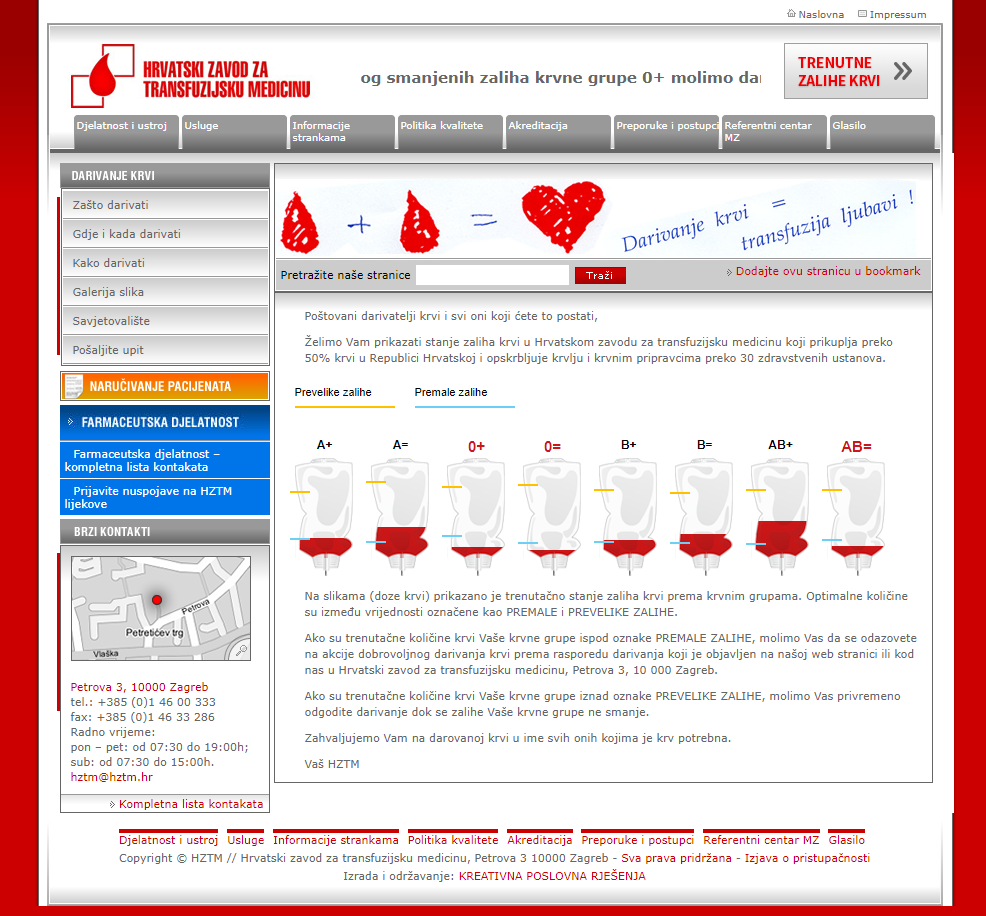
\includegraphics[scale=0.6]{slike/hztm-stranica.PNG}
			\centering
			\caption{Postojeća stranica HZTM-a}
			\label{fig:hztm-stranica}
		\end{figure}
        
        \section{Odabir tehnologije}
        
            \par {Aplikacija je izrađena u razvojnom okviru\textit{ Java Spring Boot} s poslužiteljske strane, a u \textit{Reactu} sa klijentske strane. Za pohranu, organizaciju i pristup podacima sustav koristi PostgreSQL bazu podataka pokrenutu u Docker spremniku. Aplikacija je puštena u pogon preko javno dostupne cloud platforme Heroku. Navedeni razvojni okviri nude sve funkcionalnosti potrebne za izradu opisanog sustava, što će biti detaljnije opisano u poglavlju \ref{arhitektura} i u drugoj reviziji u poglavlju \textit{Implementacija}. \\}
            %Umetnuti referencu u 2. ciklusu
            
        \section{Detaljan opis sustava}
        
            \par{
            Aplikaciji mogu pristupiti i prijavljeni i neprijavljeni korisnici koji imaju različite ovlasti u sustavu.
            \\
            Neprijavljeni korisnici imaju uvid u trenutne razine zaliha krvi i mogućnost prijaviti se ili se registrirati te time steći ovlasti prijavljenog korisnika.
            \\
            Prijavljeni korisnici po razini ovlasti dijele se na donore, djelatnike banke i administratore.
            }
             \par{
            Donori se mogu registrirati samostalno i prije darivanja krvi na javnoj stranici aplikacije. Ako im račun pak stvori djelatnik banke na prvom darivanju krvi, donori ne moraju prolaziti kroz proces registracije, već se prijavljuju s postojećim podatcima. 
            }
             \par{
            U svakom slučaju, pri stvaranju bilo kojeg računa u sustavu na e-adresu šalje se poruka s generiranim identifikatorom, inicijalnom lozinkom i poveznicom za aktivaciju. Nakon pristupa poveznici za aktivaciju, račun je aktiviran i može se koristiti.
            }
             \par{
            Nakon prijave u sustav, donori imaju pristup svim prošlim pokušajima darivanja krvi, imaju uvid u trenutno stanje zalihe njihove krvne grupe i imaju mogućnost izmijeniti neki od matičnih ili kontakt podataka svog računa (kao npr. adresu, broj telefona, e-adresu i sl.). Donori ne mogu mijenjati zdravstvene podatke računa, kao što su krvna grupa i trajno odbijanje. Donorima se također nudi mogućnost preuzimanja potvrde o bilo kojem prijašnjem darivanju krvi.
            }
             \par{Djelatnici banke prijavom u sustav mogu mijenjati svoje matične i kontakt podatke, uređivati sve podatke donora, evidentirati slanje određenog broja doza krvi u vanjsku instituciju (bolnicu) te evidentirati novi pokušaj darivanja krvi. Pri evidenciji pokušaja darivanja, koji se tipično radi na akciji darivanja krvi, djelatnik banke evidentira potrebne zdravstvene podatke kao i uspješnost pokušaja darivanja te, ukoliko zabilježeni podatci sadrže neke od podataka koji to impliciraju, evidentira trajno odbijanje donora u njegovom računu.
            }
            \par{
            Administratori sustava u sustavu imaju ovlast kreirati nove račune djelatnika banke, deaktivirati bilo koji račun u sustavu (u slučaju pogrešnog stvaranja, smrti ili prekida radnog odnosa) te definirati optimalne razine zaliha krvi za svaku krvnu grupu. Optimalne razine služe svim korisnicima sustava da jednostavnije zaključe značenje trenutnih zaliha krvi. Optimalne granice također služe i za okidanje slanja upozorenja korisnicima sustava. 
            }
            \par{
            Kada razina zalihe krvi pojedine krvne grupe padne ispod donje optimalne granice, svi djelatnici banke u sustavu dobivaju upozorenje o tome, a upozorenje dobivaju i zabilježeni donori te krvne grupe.\\
            Upozorenje se izdaje i prijelazom gornje optimalne granice, ali samo djelatnicima banke. \\
            Donori pak dodatnu obavijest dobivaju kada istekne njihov period zabrane darivanja. Naime, iz zdravstvenih razloga, donori ne smiju prečesto darivati krv, pa za muškarce minimalni period između dva darivanja krvi iznosi tri mjeseca, a za žene četiri mjeseca. Kako donori ne bi zaboravili na istek tog perioda zabrane, sustav im po isteku tog perioda šalje obavijest.
            }
            \par{
            S obzirom na to da se pri stvaranju bilo kojeg računa lozinka generira automatski, svi prijavljeni korisnici sustava imaju mogućnost promijeniti svoju lozinku u nešto što će lakše zapamtiti.
            }
        
        \section{Prepoznati i razriješeni rizici}
            \par{
            Mnogi rizici u radu sustava i njegovom korištenju prepoznati su unaprijed i razriješeni. Neki rizici proizlaze iz domene primjene, a neki iz predviđanja nesavršenog ponašanja u radu sa sustavom. Neki od prepoznatih rizika i njihova implementirana rješenja ili razlozi odbacivanja su:
            }
            \begin{itemize}
                \item Korisnik sustava zaboravlja svoj userId (donorId, bankworkerId) iako već ima stvoren račun
                \begin{itemize}
                    \item U e-poruci s poveznicom za aktivaciju navedeni su i donorId i inicijalna lozinka, pa se korisnik pronalaskom aktivacijske poruke može podsjetiti zaboravljenih podataka
                    \item Djelatnik banke donora i administrator djelatnika banke može pretražiti po bilo kojoj kombinaciji podataka, npr. imena, prezimena ili OIB-a. Na taj način može se pronaći račun u sustavu i podsjetiti donorIdja.
                \end{itemize}
                
                \item Donor pri stvaranju računa nema neki podatak
                \begin{itemize}
                    \item Kao obavezni podatci označeni su samo oni koje bi većina ljudi trebala znati ili imati uvijek dostupno
                    \item Ako donor račun stvara samostalno, uvijek može odgoditi stvaranje računa dok ne pronađe obavezni podatak koji mu nedostaje
                    \item Neobavezni podatci ne moraju se unijeti pri stvaranju računa pa ih donor može unijeti i kasnije prijavom u sustav, ili pri idućem doniranju
                \end{itemize}
                
                \item Podatci koji se unesu za donora mogu zabunom biti semantički neispravni (tipfeleri pri unosu adrese, broja telefona, ...) što validacija sustava ne može prepoznati
                \begin{itemize}
                    \item Pri svakom doniranju, djelatnik banke provjerava unesene podatke s donorom te ih popravlja u slučaju greške
                    \item Donor pogrešne podatke može i samostalno ispraviti prijavom u sustav i pregledom osobnih podataka
                \end{itemize}
                
                \item Sustav se može zablokirati zbog neadekvatnog sklopovlja pa se neke aktivnosti ne mogu pravovremeno obaviti
                \begin{itemize}
                    \item U ovakvom ekstremnom slučaju može se ručno voditi evidencija podataka koji su neophodni za obaviti trenutno dok se problem ne riješi pa se podatci unesu naknadno, a aktivnosti koje nije nužno obaviti u istom trenutk mogu se odgoditi do oporavka sustava
                \end{itemize}
                
                \item Baza podataka pri pokušaju unosa nema dovoljno prostora za pohranu novih zapisa
                \begin{itemize}
                    \item Sustav je dovoljno malen da ovo odstupanje ne predstavlja značajan rizik
                    \item Administrator sustava mogao bi s vremena na vrijeme voditi računa o popunjenosti diska s bazom podataka i tako na vrijeme spriječiti nastanak opisane situacije
                    \item Rizik se može na vrijeme spriječiti većom investicijom u opremu
                \end{itemize}
                
                \item Neovlašteni korisnik može nasumično pogoditi aktivacijsku poveznicu i aktivirati račun bez dopuštenja
                \begin{itemize}
                    \item Aktivacijska poveznica dovoljno je dugačka da ovo ne predstavlja značajan rizik
                \end{itemize} 
                
                \item Djelatnik banke želi promijeniti donorId nekog donora, a donorId je primarni ključ u bazi podataka (isto vrijedi i za odnos administrator - djelatnik banke)
                \begin{itemize}
                    \item Primarni ključevi samo se ispisuju na ekran pri pregledu i uređivanju podataka računa i ne mogu se mijenjati.
                    \item Nije prepoznata funkcionalno nužna situacija kada bi ova funkcionalnost bila potrebna, osim iz \textit{estetskih} razloga 
                \end{itemize}
                
                \item Djelatnik banke na doniranju pogrešno tumači neki zdravstveni podatak i pogrešno evidentira trajno odbijanje donora koji ne bi trebao biti trajno odbijen
                \begin{itemize}
                    \item Trajno odbijanje, kao i ostali podatci, može se naknadno ispraviti u sustavu ako se ispostavi da je riječ o pogrešci
                \end{itemize}
                
                \item Donor prešućuje neki od podataka zbog kojih ne bi trebao moći darivati krv
                \begin{itemize}
                    \item Sustav nikako ne može otkriti ovu informaciju, već je ovo problem iz domene primjene (koji je većinom riješen time da se doniranje krvi ne plaća i da se ampula krvi dodatno testira na krvnu grupu i patogene)
                \end{itemize}
                
            \end{itemize}
        
        
        \section{Ograničenja u implementaciji}
            
            \par{
            S obzirom na ograničen vremenski rok i ograničene resurse za izradu sustava, na brojnim mjestima u dogovoru s asistentom dogovoren je nužan i dovoljan opseg rješenja. Taj opseg definiran je funkcionalnim i nefunkcionalnim zahtjevima, dok su dodatne stvari ostavljene na slobodu timu za implementaciju.
            }
            \par{
            Dio problema sa sustavom proizlazi iz ograničenih resursa dostupnih za puštanje aplikacije u pogon na besplatnom servisu \textit{Heroku}, koji gasi aplikaciju nakon određenog vremena u kojemu ne primi nijedan zahtjev. Zbog toga neke funkcionalnosti (poput slanja obavijesti o ponovnoj mogućnosti darivanja) neće raditi pouzdano. Kako bi se ove funkcionalnosti ispitale treba prvo napraviti neki zahtjev i na klijentski poslužitelj i na poslužitelj poslužiteljske aplikacije kako bi se oni pokrenuli, a nakon toga u redovnom korištenju aplikacije ne bi trebalo biti problema. Kako se obavijest o ponovnoj mogućnosti darivanja šalje svaki dan u 12:00 za sve donore koji su donirali krv tri/četiri mjeseca ranije, radi ispitivanja potrebno je netom prije 12:00 poslati bilo kakav zahtjev poslužiteljskoj aplikaciji kako bi se ona pokrenula (i naravno, imati donora u sustavu kojemu na taj dan istječe period nemogućnosti darivanja).
            }
            \par{
            Potencijalan problem predstavlja i servis e-pošte, koji u nekom trenutku može onemogućiti korištenje njegovih usluga zbog sigurnosnih razloga (previše poruka i slično). Oba problema bila bi riješena posjedovanjem vlastitog poslužitelja koji bi aplikaciju držao stalno upaljenom i na kojemu bi se mogao pokrenuti vlastiti servis za e-poruke.
            }
            \par{
            Pri izradi sustava razmatrane su brojne dodatne i alternativne mogućnosti i scenariji koji u ovoj inačici aplikacije nisu podržane. Takve mogućnosti dokumentirane su u sljedećem odjeljku pa se u nekoj od budućih implementacija sustav može nadograditi da podržava neke od navedenih alternativnih mogućnosti. Te mogućnosti najčešće uključuju mogućnosti koje bi olakšale korisnicima korištenje sustava i dale dodatne funkcionalnosti koje se trenutno mogu izvoditi zaobilazno ili se zasad uopće ne mogu izvodti.
            }
        
        \section{Mogućnosti za nadogradnju}
            \par{
            S obzirom na prepoznate rizike vezane za olakšanje korištenja sustava i izvođenje dosad nemogućih radnji, osmišljene su sljedeće mogućnosti za buduću nadogradnju:
            \begin{itemize}
            
                 \item Korisnik sustava pri stvaranju računa ima zabilježenu pogrešnu e-adresu pa ne dobije poruku s aktivacijskom poveznicom, a novi račun ne može stvoriti jer su u sustavu već zabilježeni podatci koji moraju biti jedinstveni 
                 \\ ILI
                \\ Korisnik je zagubio poruku s aktivacijskom poveznicom i donorId-jem prije aktivacije računa (ili ju nije primio zbog prepunjene memorije pretinca e-pošte)
                \begin{itemize}
                    \item Moguća je nadogradnja koja  bi djelatniku banke / administratoru pri pregledu računa donora / djelatnika banke ostavila mogućnost ponovnog slanja poruke s aktivacijskom poveznicom uz eventualni ispravak e-adrese
                    \item Moguća je nadogradnja koja bi ostavila mogućnost stvaranja novog računa s istim podatcima sve dok se račun ne aktivira te bi se neaktivirani račun s istim podatcima automatski obrisao
                \end{itemize}
                
                 \item Korisnik sustava želi ostati prijavljen odmah po otvaranju aktivacijske poveznice, bez ponovnog upisa podataka za prijavu
                \begin{itemize}
                    \item Iako je ovo samo jednokratno produljenje procesa koje ne utječe značajno na iskustvo korisnika (koji, ako ima aktivacijsku poveznicu, sigurno ima i podatke za prijavu jer se nalaze u istoj poruci), moguća je nadogradnja koja bi stvorila sjednicu korisnika odmah nakon pristupa poveznici za aktivaciju
                \end{itemize}
                
                 \item Administrator zabunom deaktivira račun nekog korisnika sustava
                \begin{itemize}
                    \item Moguća je nadogradnja koja bi administratoru omogućila reaktivaciju nekog računa u sustavu
                \end{itemize}
                
                \item Donor svoju krvnu grupu može ne znati unaprijed, a u sustavu je pretpostavljeno da se podatak može odmah otkriti iako je uobičajena praksa da se krv testira naknadno
                \begin{itemize}
                    \item Krvna grupa može ostati nepopunjena pa se popuniti nakon što se obavi test na bilo koji način
                \end{itemize}
                
                \item Doza krvi na serološkom testiranju može završiti kao nepovoljna i mora se odbaciti
                \begin{itemize}
                    \item Moguća je nadogradnja gdje bi u sustavu postojala i evidencija pojedinih doza krvi koje se onda mogu evidentirati kao nepovoljne i povezati s donorima
                    \item Trenutno moguće rješenje je vođenje evidencije o dozama van sustava i ručno povezivanje s donorima
                \end{itemize}
                
                \item Administrator nije definirao optimalne granice zaliha pa stanje zaliha ne prikazuje podatke koji vizualno imaju korisno značenje
                \begin{itemize}
                    \item Moguća je nadogradnja u kojoj bi sustav administratoru slao upozorenja dok ne definira granice
                \end{itemize}
                
                \item Korisnik sustava zaboravio je lozinku pa ne može pristupiti računu
                \begin{itemize}
                    \item Moguća je nadogradnja koja bi, u slučaju promijenjene lozinke koja se ne može pronaći u e-poruci s aktivacijskom poveznicom, omogućila promjenu lozinke putem e-adrese koja je navedena u računu ili slanje postojeće lozinke na tu e-adresu  
                \end{itemize}
                
                \item Donor želi potvrdu o doniranju poslanu na e-adresu umjesto preuzimanja
                \begin{itemize}
                    \item Moguća je nadogradnja koja bi uz preuzimanje ponudila i mogućnost slanja potvrde na e-adresu, vrlo slično aktivnosti opisanoj u koraku 8 obrasca uporabe \hyperref[UC6]{UC6}
                \end{itemize}
                
                \item Donor želi potvrdu o doniranju i za neuspješan pokušaj doniranja
                \begin{itemize}
                    \item Moguća je nadogradnja koja bi omogućila generiranje PDF potvrde za sve pokušaje doniranja, ne samo za uspješne
                \end{itemize}
                
                \item U sustavu je zabilježena pogrešna e-adresa donora na koju će se slati poruka s aktivacijskom poveznicom i PDF potvrde o doniranjima
                \begin{itemize}
                    \item PDF potvrda ne sadrži nikakve osjetljive podatke pa ona ne predstavlja značajan rizik za slanje na tuđu e-adresu
                    \item Na idućem doniranju krvi moguće je izmijeniti e-adresu na koju će se slati potvrde i (kako je već opisano u jednoj od prethodnih dodatnih mogućnosti) poslati novu aktivacijsku poveznicu
                \end{itemize}
                
                \item Stanje zaliha krvi u sustavu nije u skladu sa stanjem zaliha u skladištu
                \begin{itemize}
                    \item Moguća je nadogradnja koja bi administratoru omogućila \textit{rekalibraciju} stanja (trenutno se problem djelomično riješiti ručnim smanjivanjem stanja zaliha krvi) 
                \end{itemize}
                
                \item Čestim slanjem doza krvi u bolnice i novim doniranjem može doći do čestog prelaska donje granice i prečestog slanja obavijesti
                \begin{itemize}
                    \item Moguća je nadogradnja koja bi uvela period vremena u kojemu se korisnicima ne bi slale poruke češće od npr. svaka dva dana
                \end{itemize}
                
                \item Donori koji su donirali krv u posljednja 3/4 mjeseca nikako ne mogu ponovno donirati krv i obavijest im je uglavnom nepotrebna
                \begin{itemize}
                    \item Moguća je nadogradnja koja bi zaustavila slanje obavijesti o nedostatku krvi za vrijeme nedopuštenog perioda darivanja
                    \item Moguća je nadogradnja koja bi omogućila potpunu odjavu s upozorenja
                \end{itemize}
                
                \item Baza podataka može propustiti stvoriti okidač za slanje upozorenja donorima kojima je upravo istekao nedopušteni period darivanja
                \begin{itemize}
                    \item Iako svatko može na profilu vidjeti kada je zadnji put darivao krv, moguća je nadogradnja koja bi za svakog donora čuvala je li mu poslano upozorenje ili ne (koje bi se resetiralo na \textit{ne} pri svakom novom doniranju), pa bi se onda upozorenje slalo svim korisnicima kojima je prošlo \underbar{više} od 3 ili 4 mjeseca od prošlog darivanja, a obavijest im nije poslana (pa bi se proces slanja mogao pokretati i rjeđe)
                \end{itemize}
                
                \item S obzirom na potencijalne zainteresirane strane kao što je zavod za javno zdravstvo, nepraktično je što sustav nije povezan s postojećim sustavima koji se koriste u zdravstvu
                \begin{itemize}
                    \item Sustav bi u budućoj implementaciji mogao podržati i spajanje s postojećim sustavima koji se već uhodano koriste u zdravstvu. Tako bi se obogatile funkcionalnosti oba softvera i stvorilo još veće rasterećenje zdravstvenom sustavu.
                \end{itemize}
                
                \item Jedan administrator u sustavu mogao bi biti nedovoljan za obavljanje posla administracije računa
                \begin{itemize}
                    \item Sustav bi u budućoj implementaciji mogao podržati stvaranje novog računa administratora pa bi se tako posao mogao podijeliti na više osoba
                \end{itemize}
                
                \item Korisnici bi mogli htjeti promijeniti inicijalnu lozinku, bilo radi lakšeg pamćenja, ili zbog sigurnosti
                \begin{itemize}
                    \item Sustav bi u budućoj implementaciji mogao podržati promjenu lozinke - funkcionalnost već postoji sa poslužiteljske strane, ali se može napraviti i sa klijentske strane
                \end{itemize}
                
            \end{itemize}
            }
            
\begin{comment}
        
		\section{Primjeri u \LaTeX u}
		
		\textit{Ovo potpoglavlje izbrisati.}\\

		U nastavku se nalaze različiti primjeri kako koristiti osnovne funkcionalnosti \LaTeX a koje su potrebne za izradu dokumentacije. Za dodatnu pomoć obratiti se asistentu na projektu ili potražiti upute na sljedećim web sjedištima:
		\begin{itemize}
			\item Upute za izradu diplomskog rada u \LaTeX u - \url{https://www.fer.unizg.hr/_download/repository/LaTeX-upute.pdf}
			\item \LaTeX\ projekt - \url{https://www.latex-project.org/help/}
			\item StackExchange za Tex - \url{https://tex.stackexchange.com/}\\
		
		\end{itemize} 	


		
		\noindent \underbar{podcrtani tekst}, \textbf{podebljani tekst}, 	\textit{nagnuti tekst}\\
		\noindent \normalsize primjer \large primjer \Large primjer \LARGE {primjer} \huge {primjer} \Huge primjer \normalsize
				
		\begin{packed_item}
			
			\item  primjer
			\item  primjer
			\item  primjer
			\item[] \begin{packed_enum}
				\item primjer
				\item[] \begin{packed_enum}
					\item[1.a] primjer
					\item[b] primjer
				\end{packed_enum}
				\item primjer
			\end{packed_enum}
			
		\end{packed_item}
		
		\noindent primjer url-a: \url{https://www.fer.unizg.hr/predmet/proinz/projekt}
		
		\noindent posebni znakovi: \# \$ \% \& \{ \} \_ 
		$|$ $<$ $>$ 
		\^{} 
		\~{} 
		$\backslash$ 
		
		
		\begin{longtblr}[
			label=none,
			entry=none
			]{
				width = \textwidth,
				colspec={|X[8,l]|X[8, l]|X[16, l]|}, 
				rowhead = 1,
			} %definicija širine tablice, širine stupaca, poravnanje i broja redaka naslova tablice
			\hline \multicolumn{3}{|c|}{\textbf{naslov unutar tablice}}	 \\ \hline[3pt]
			\SetCell{LightGreen}IdKorisnik & INT	&  	Lorem ipsum dolor sit amet, consectetur adipiscing elit, sed do eiusmod  	\\ \hline
			korisnickoIme	& VARCHAR &   	\\ \hline 
			email & VARCHAR &   \\ \hline 
			ime & VARCHAR	&  		\\ \hline 
			\SetCell{LightBlue} primjer	& VARCHAR &   	\\ \hline 
		\end{longtblr}
		

		\begin{longtblr}[
				caption = {Naslov s referencom izvan tablice},
				entry = {Short Caption},
			]{
				width = \textwidth, 
				colspec = {|X[8,l]|X[8,l]|X[16,l]|}, 
				rowhead = 1,
			}
			\hline
			\SetCell{LightGreen}IdKorisnik & INT	&  	Lorem ipsum dolor sit amet, consectetur adipiscing elit, sed do eiusmod  	\\ \hline
			korisnickoIme	& VARCHAR &   	\\ \hline 
			email & VARCHAR &   \\ \hline 
			ime & VARCHAR	&  		\\ \hline 
			\SetCell{LightBlue} primjer	& VARCHAR &   	\\ \hline 
		\end{longtblr}
	

		
		%unos slike
		\begin{figure}[H]
			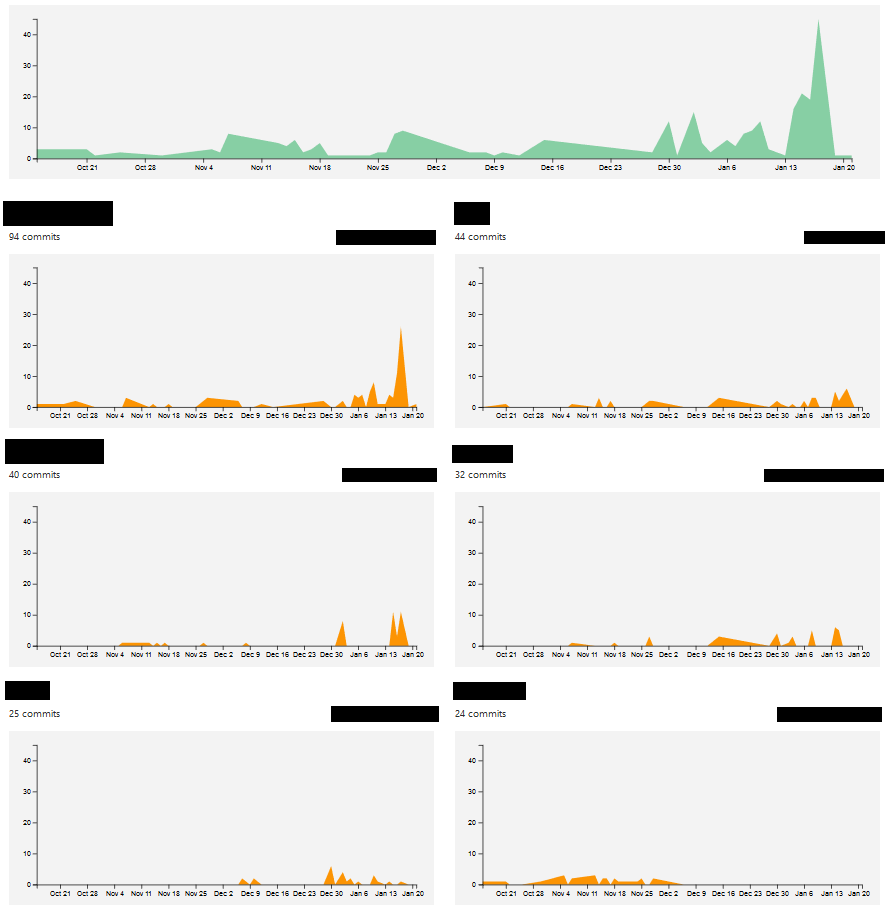
\includegraphics[scale=0.4]{slike/aktivnost.PNG} %veličina slike u odnosu na originalnu datoteku i pozicija slike
			\centering
			\caption{Primjer slike s potpisom}
			\label{fig:promjene}
		\end{figure}
		
		\begin{figure}[H]
			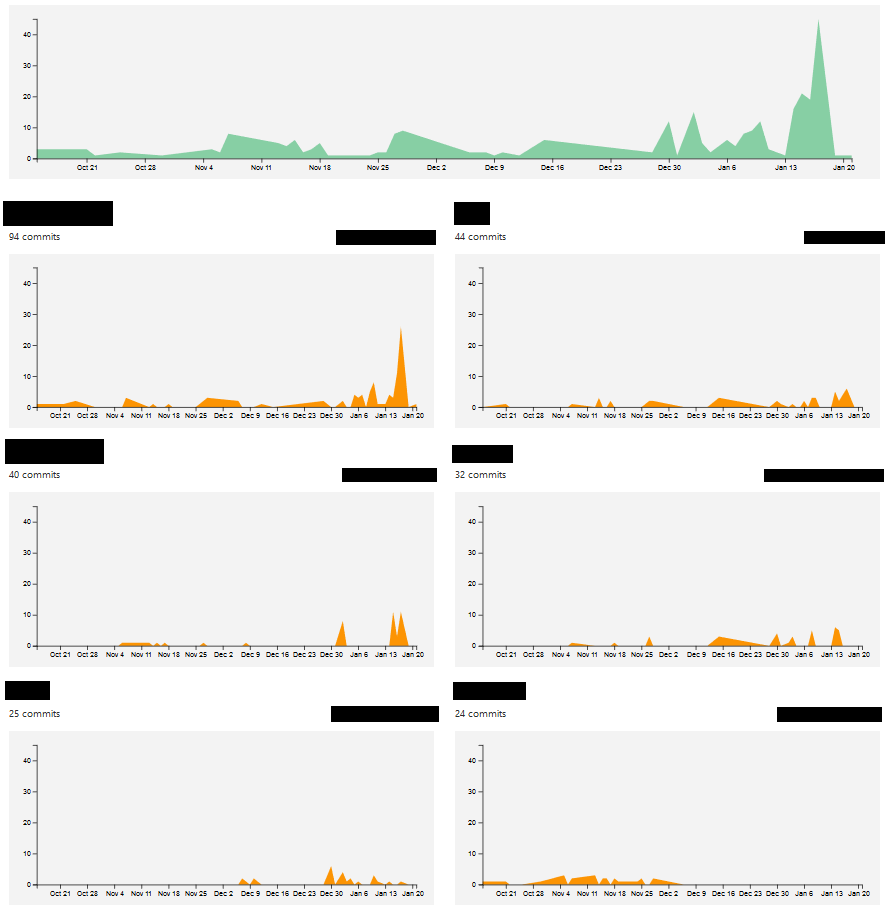
\includegraphics[width=\textwidth]{slike/aktivnost.PNG} %veličina u odnosu na širinu linije
			\caption{Primjer slike s potpisom 2}
			\label{fig:promjene2} %label mora biti drugaciji za svaku sliku
		\end{figure}
		
		Referenciranje slike \ref{fig:promjene2} u tekstu.
		
\end{comment}
		\eject
		
	